\documentclass[11pt, oneside]{article} 
\usepackage{geometry}
\geometry{letterpaper} 
\usepackage{graphicx}
	
\usepackage{amssymb}
\usepackage{amsmath}
\usepackage{parskip}
\usepackage{color}
\usepackage{hyperref}

\graphicspath{{/Users/telliott_admin/Tex/png/}}
% \begin{center} 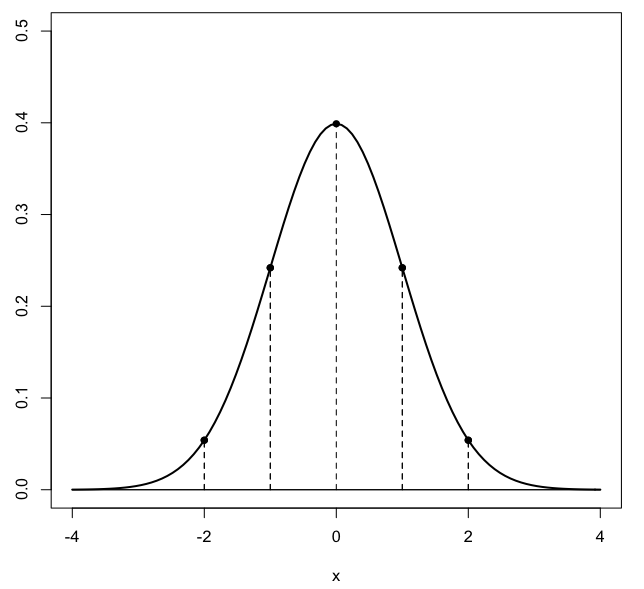
\includegraphics [scale=0.4] {gauss3.png} \end{center}

%break
\title{Lagrange}
\date{}

\begin{document}
\maketitle
\Large
This chapter is about the method of Lagrange multipliers.  We have a function $f(x,y)$ and we want to maximize it, but the variables are not independent, e.g. $g(x,y) = c$ where $c$ is a constant.  Let's work an example and then come back to the justification afterward.

\subsection*{example}
\url{https://gravityandlevity.wordpress.com/2018/07/06/lagrange_multipliers/}

\begin{quote}You are living on an inclined plane described by the equation $z = -2x + y$, but you can only move along the circle described by $x^2 + y^2 = 1$. What is the highest point
(largest $z$) that you can reach? What is the lowest point?\end{quote}

\begin{center} 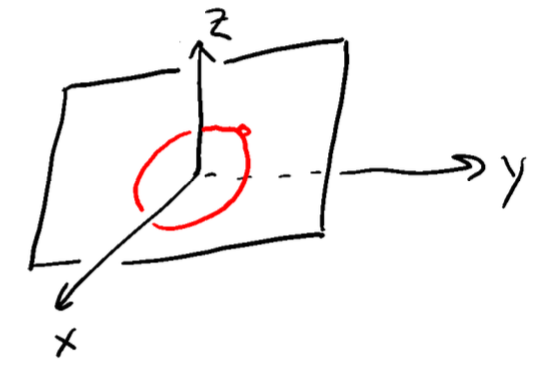
\includegraphics [scale=0.4] {Lagrange_max.png} \end{center}

\subsection*{example 0}

\[ f(x,y) = -2x + y \]
\[ g(x,y) = x^2 + y^2 = 1 \]
So
\[ f_x = -2 = \lambda g_x = \lambda(2x) \]
\[ f_y = 1 = \lambda g_y = \lambda(2y) \]
Then
\[ x = -\frac{1}{\lambda} \]
\[ y = \frac{1}{2\lambda} \]

Use the constraint to solve for $\lambda$:
\[ \frac{1}{\lambda^2} + \frac{1}{4 \lambda^2} = 1 \]
\[ \frac{5}{4\lambda^2} = 1 \]
\[ \lambda = \pm \frac{\sqrt{5}}{2} \]
Solve for $x$ and $y$.  The maximum occurs when
\[ x = -\frac{2}{\sqrt{5}}, \ \ \ \ y = \frac{1}{\sqrt{5}} \]
\[ f(x,y) = \frac{5}{\sqrt{5}} = \sqrt{5} \]

\subsection*{alternative}

An alternative approach not using the method would be to solve the constraint to eliminate one variable, like this:
\[ y = \sqrt{1 - x^2} \]
so
\[ f(x,y) = -2x + \sqrt{1 - x^2} \]
Take the derivative and set it equal to zero
\[ f_x = -2 + \frac{1}{2} \ \frac{1}{ \sqrt{1 - x^2}} \ (-2x) = 0 \]
\[ \frac{x}{ \sqrt{1 - x^2}} = -2 \]
\[ x^2 = 4(1-x^2) \]
\[ 5x^2 = 4 \]
\[ x = \pm \frac{2}{\sqrt{5}} \]

This is not so easy in general because the derivative usually gets messy.

\subsection*{idea}
According to 

\url{https://gravityandlevity.wordpress.com/2018/07/06/lagrange_multipliers/}

\begin{quote} The key idea behind the method of Lagrange multipliers is that, instead of trying to reduce the number of variables, you increase the number of variables by adding a set of unknown constants (called Lagrange multipliers). What you get in exchange for increasing the number of variables, however, is a new function (commonly denoted $\Lambda$), for which all the variables are independent. With this magic new function you can do the optimization simply by taking the derivative of $\Lambda$Λ with respect to each variable one at a time. This function (called the Lagrange function) is:\end{quote}

\[ \Lambda(x,y,\lambda) = f(x,y) - \lambda \ g(x,y) \]

where $g(x,y)$ is the constraint rewritten with everything on the left-hand side.  In this example:
\[ x^2 + y^2 - 1 = 0 \]
so
\[ \Lambda(x,y,\lambda) = -2x + y - \lambda (x^2 + y^2 - 1) \]
In the function $\Lambda$, $x$ is no longer dependent on $y$, and taking the derivatives is simple.

Set equal to zero, these are:
\[ \Lambda_x = -2 - 2\lambda x = 0 \]
\[ \Lambda_y = 1 - 2\lambda y = 0 \]
\[ \Lambda_\lambda = - (x^2 + y^2 - 1) = 0 \]

The third equation is just the constraint.  But the first two equations are just what we had before.  Solve for $x$ and $y$ and plug into $g(x,y)$ to obtain $\lambda$ and it's exactly the same.

\subsection*{summary of the method}

Another way to say this is that the method of Lagrange multipliers finds a solution to this equation
\[ \nabla f = \lambda \nabla g \]

If there is a constrained max (or min), it will satisfy this equation.  In words, we can say that at a point which satisfies the constraint $g(x,y) = c$, and maximizes or minimizes $f(x,y)$, the gradients of the two functions are equal, within some constant $\lambda$. 

\subsection*{example 1}

Suppose

\[ f(x,y) = xy \]
\[ g(x,y) = x + y = 10 \]

This could be the famous maximum area problem where $x$ and $y$ are the sides of a rectangle, the semiperimeter is given, and the objective is to pick $x$ and $y$ to maximize the area.  We see a solution for this in Calculus 1, namely, solve $g$ for one of the variables.

\[ x = 10 - y \]
and substitute:
\[ h(y) = (10-y)y = 10y - y^2 \]
\[ h'(y) = 10 - 2y = 0 \]
\[ h''(y) = - 2 \]
Since the second derivative is $< 0$, this is a maximum, and the solution is $y = 5, x = 5$.

Using the Lagrange method we say
\[ \nabla f = \lambda \nabla g \]
\[ f_x = \lambda g_x \]
\[ f_y = \lambda g_y \]
Plugging in, we obtain two equations

\[ f_x = y = \lambda g_x = \lambda \]
\[ f_y = x = \lambda g_y = \lambda \]
So, clearly $x=y$.

\subsection*{example 2}

Corral gives this problem.  Find the points on the circle $x^2 + y^2 = 80$ that are either closest to or furthest from the point $P = (1,2)$.

The circle equation is the constraint.  We need to find an equation for distance, which we will then maximize.
\[ d = \sqrt{(1-x)^2 + (2-y)^2} \]

We can simplify by saying that when $d^2$ is a min or a max, so is $d$.  So now we have

\[ f(x,y) = d^2 = (1-x)^2 + (2-y)^2 = 1 - 2x + x^2 + 4 - 4y + y^2 \]
\[ f_x = -2 + 2x \]
\[ f_y = -4 + 2y \]
\[ g_x = 2x \]
\[ g_y = 2y \]

So 
\[ \nabla f = \lambda \nabla g \]
\[ f_x = \lambda g_x \]
\[ f_y = \lambda g_y \]
Plugging in, we obtain two equations

\[ -2 + 2x = \lambda 2x \]
\[ -4 + 2y = \lambda 2y \]
Solve for $\lambda$ and set them equal

\[ \frac{-4 + 2y}{2y} = \frac{-2 + 2x}{2x} \]
\[ \frac{-2 + y}{y} = \frac{-1 + x}{x} \]
\[ -2x + xy = -y + xy \]
\[ y = 2x \]

Since $x^2 + y^2 = 80$
\[ x^2 + 4x^2 = 80 \]
and so $x= \pm 4$ and the solutions are $(4,8)$, $(-4,-8)$.  Here is the diagram from Corral

\begin{center} 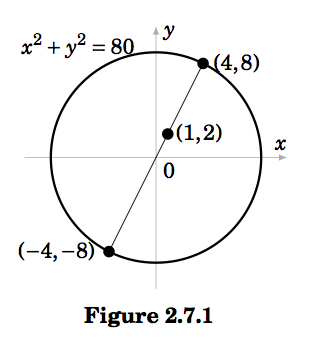
\includegraphics [scale=0.5] {Corral1.png} \end{center}

\subsection*{example 3}
Consider the inverted paraboloid 
\[ z = x^2 + y^2 \]
Now ask, which values $(x,y)$ give a maximum (or minimum) value on the surface, that are also on the line $y = 1 + x$?

Try to visualize what we're asking here.  We have as our surface a kind of elongated and inverted bowl, with its vertex at the origin, opening up.  The vertical plane that cuts through the $x,y$-plane along the given line traces out a curve in its intersection with the surface.  

Since the line is symmetric with respect to the origin and the surface is also, I predict that the answer will be that $x = y$.  Let's see.
\[ f(x,y) = x^2 + y^2 \]
\[ \nabla f = \langle \ 2x, 2y \rangle \]
Be sure to re-cast the line equation as a function $g(x,y)$:
\[ g(x,y) = y - x = 1 \]
\[ \nabla g = \langle \ -1, 1 \rangle \]
So we have that
\[ \lambda \ \nabla f = \nabla g \]
This is two equations:
\[ -2x \lambda = 1 \]
\[ 2y \lambda = 1 \]
\[ -\frac{1}{2x} = \frac{1}{2y} \]
\[ -x = y \]
Go back to $g$ to plug in and solve for $x$:
\[ - x - x = 1, \ \ \ x = - \frac{1}{2} \]
and
\[ y = -x = - - \frac{1}{2} = \frac{1}{2} \]
The answer is as predicted.

\subsection*{example 4}

Here is one from Paul's \emph{Calculus}.  Find the dimensions of a rectangular box with maximum volume, subject to the constraint that the surface area is fixed.

\[ V = xyz \]
\[ A = 2(xy + xz + yz) = \text{constant} \]
Now
\[ \nabla V = \ <f_x,f_y,f_z> \]
we have then three equations plus a fourth (the one for area above).
\[ f_x = \lambda g_x = yz = 2 \lambda (y+z) \]
\[ f_y = \lambda g_y = xz = 2 \lambda (x+z) \]
\[ f_z = \lambda g_z = xy = 2 \lambda (x+y) \]
Paul uses a nice trick to solve this.  Take the first two equations, multiply eqn. 1 by x and eqn. 2 by y:
\[ xyz = 2 \lambda x(y+z) \]
\[ xyz = 2 \lambda y(x+z) \]
\[ xy + xz = xy + yz \]
\[ x = y \]
By symmetry, $x=y=z$.

\subsection*{example 5}

Auroux gives this problem:  on the curve of the hyperbola $xy=3$, find the point closest to the origin.

The distance to the origin is 
\[ d = \sqrt{x^2 + y^2} \]
but we can again simplify things a bit because if $d^2$ is a minimum, then $d$ is a minimum.  So the function we need to minimize is

\[ f(x,y) = x^2 + y^2 \]
subject to the constraint $xy = 3$.

The graph of $f(x,y)$ is a \emph{surface}---a paraboloid with circular cross-section---with apex at $(0,0,0)$, and opening up.  $x^2 + y^2$ is a \emph{level curve} of $f$, at the value $f=a$.

In this figure we have the situation as described, except that  $xy = 1/2$.
\begin{center}
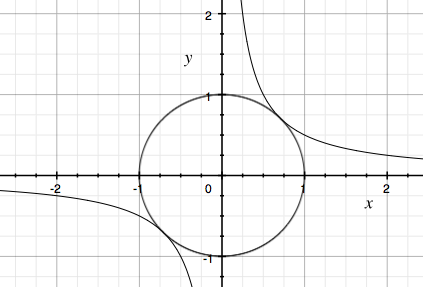
\includegraphics [scale=0.5] {lagrange.png}
\end{center}

The idea of the method is that, at the maximum, the circle just touches the hyperbola.  And at the point of contact, the gradient of the circle function is parallel to the gradient of the hyperbola function, so the two are equal when one is multiplied by a constant that is usually designated $\lambda$.
\[ \nabla f = \lambda \nabla g \]

We have
\[ f(x,y) = x^2 + y^2 \]
\[ f_x = 2x \]
\[ f_y = 2y \]
\[ g(x,y) = xy = c \]
\[ \nabla f = \lambda \nabla g \]

so the two equations we get are
\[ 2x - \lambda y = 0 \]
\[ \lambda x - 2y = 0 \]
Auroux uses some linear algebra trickery to solve this.  A matrix equation $A\mathbf{v}=\mathbf{0}$ has solutions other than $\mathbf{v}=0$ only if det(A) = 0.  So that's what we do:
\[ A =
\begin{bmatrix} 
  2  &  -\lambda   \\ 
  \lambda  &  -2  
\end{bmatrix}
\]
The determinant is
\[ -4 + \lambda^2 = 0 \]
\[ \lambda = \pm 2 \]
Using $2x - \lambda y = 0$,for $\lambda = 2$, we obtain $2x-2y=0$ and $x=y$, while for $\lambda = -2$, we obtain $2x+2y=0$ and $x=-y$.  Exactly as you would predict from the figure.  

\end{document}  